%!TEX root = ../presentation.tex

\chapter{Rust in Depth}
\label{chap_rv}
\targets{
  \item See some of Rust's concepts in practical examples.
  \item Learn more about ownership, borrowing and lifetime.
  \item Get to know some of Rust's error messages.
  \item Be able to write small Rust programs.
}

\section{Mutability}

\subsection{Concurrent Iterator Modification}

\lstset{basicstyle=\ttfamily\scriptsize,frame=none,backgroundcolor={}}

\begin{Frame}[fragile]{Concurrent Iterator Modification}{Java}
\begin{lstlisting}[language=Java]
public static void doubleList(List<Integer> list) {
    for(int x: list) {
        list.add(x); // RUNTIME ERROR!
        // ConcurrentModificationException
    }
}

public static void main(String[] args) {
    ArrayList<Integer> list = new ArrayList<>();
    list.add(1); list.add(2); list.add(3);
    doubleList(list);
}
\end{lstlisting}
\end{Frame}

\begin{Frame}[fragile]{Concurrent Iterator Modification}{Rust}
\begin{lstlisting}[language=Rust]
pub fn concurrent_modification() {
    let mut vec = vec!(1,2,3);
    for x in &vec {
        vec.push(*x); // ERROR!
        // cannot borrow `vec` as mutable
        // because it is also borrowed as immutable
    }
}
\end{lstlisting}
\end{Frame}

\subsection{Accidental Reference Modification}

\begin{Frame}[fragile]{Accidental Reference Modification}{Java}
\begin{lstlisting}[language=Java]
static int findMedian(List<Integer> numbers) {
    Collections.sort(numbers);
    int n = numbers.size();
    if (n % 2 == 0) {
        return (numbers.get(n/2) + numbers.get(n/2-1)) / 2;
    } else {
        return numbers.get(n/2);
    }
}

static void main(String[] args) {
    List<Integer> numbers = Arrays.asList(8,2,4,3);
    int median = findMedian(numbers);
    System.out.println("You entered: " + numbers);
    // => You entered: [2,3,4,8] // WRONG!
    System.out.println("The median is: " + median);
    // => The median is: 3
}
\end{lstlisting}
\end{Frame}

\begin{Frame}[fragile]{Accidental Reference Modification}{Rust: Move}
\begin{lstlisting}[language=Rust]
fn find_median_move(mut numbers: Vec<i32>) -> i32 {
    numbers.sort();
    let n = numbers.len();
    if n % 2 == 0 {
        (numbers[n/2-1] + numbers[n/2]) / 2
    } else {
        numbers[n/2]
    }
}

fn main() {
    let numbers = vec!(8,2,4,3);
    println!("You entered: {:?}", numbers);
    // => You entered: [8, 2, 4, 3]
    
    let median = find_median_move(numbers);
    
    println!("You entered: {:?}", numbers); // ERROR!
    // borrow of moved value: `numbers`

    println!("The median is: {}", median);
    // => The median is: 3
}
\end{lstlisting}
\end{Frame}

\begin{Frame}[fragile]{Accidental Reference Modification}{Rust: Copy}
\begin{lstlisting}[language=Rust]
fn find_median_ref(original_numbers: &Vec<i32>) -> i32 {
    original_numbers.sort(); // ERROR!
    // cannot borrow `*original_numbers` as mutable,
    // as it is behind a `&` reference
    
    let mut numbers = original_numbers.clone();
    numbers.sort();
    let n = numbers.len();
    if n % 2 == 0 {
        (numbers[n/2-1] + numbers[n/2]) / 2
    } else {
        numbers[n/2]
    }
}

fn main() {
    let numbers = vec!(8,2,4,3);
    let median = find_median_ref(&numbers);
    
    println!("You entered: {:?}", numbers);
    // => You entered: [8, 2, 4, 3]
    println!("The median is: {}", median);
    // => The median is: 3
}
\end{lstlisting}
\end{Frame}

\begin{Frame}[fragile]{Accidental Reference Modification}{Rust: Mutable Reference}
\begin{lstlisting}[language=Rust]
fn find_median_mut_ref(numbers: &mut Vec<i32>) -> i32 {
    numbers.sort();
    let n = numbers.len();
    if n % 2 == 0 {
        (numbers[n/2-1] + numbers[n/2]) / 2
    } else {
        numbers[n/2]
    }
}

fn main() {
    let mut numbers = vec!(8,2,4,3);
    let median = find_median_mut_ref(&mut numbers);
    
    println!("You entered: {:?}", numbers);
    // => You entered: [2, 3, 4, 8] // WRONG!
    println!("The median is: {}", median);
    // => The median is: 3
}
\end{lstlisting}

\scriptsize
Same problem as in the Java version, but now its easy to spot because we had to write
\lstinline[language=Rust]|&mut numbers| on the previous line and
\lstinline[language=Rust]|let mut numbers| on the line before it.\par
\end{Frame}

\section{Memory Management}

\subsection{Basics}

\begin{Frame}[fragile]{Basic Memory Management}{C: Returning Stack Pointers}
\begin{lstlisting}[language=C]
int* range(int from, int to) {
    int arr[from-to];
    for (int i = 0; i < from - to; i++) {
        arr[i] = from + i;
    }
    return arr; // WRONG!
    // Stack memory lives as long as the function invocation
}
\end{lstlisting}
\end{Frame}

\begin{Frame}[fragile]{Basic Memory Management}{Rust: Returning Stack Pointers}
\begin{lstlisting}[language=Rust]
fn range<'a>(from: usize, to: usize) -> &'a [usize] {
    let mut arr = [0; 1024];
    for i in 0 .. (from-to) {
        arr[i] = from + 1;
    }
    &arr // ERROR!
    // cannot return reference to local variable `arr`
}
\end{lstlisting}
\end{Frame}

\begin{Frame}[fragile]{Basic Memory Management}{C: Memory Leak}
\begin{lstlisting}[language=C]
int* range2(int from, int to) {
    int* arr = malloc((to - from) * sizeof(int));
    for (int i = 0; i < from - to; i++) {
        arr[i] = from + i;
    }
    return arr;
}

int main() {
    int* arr = range2(0, 100);
    do_something(arr);
}
// WRONG!
// Malloced memory is never freed
\end{lstlisting}
\end{Frame}

\begin{Frame}[fragile]{Basic Memory Management}{Rust: Memory Leak}
\begin{lstlisting}[language=Rust]
fn range2(from: i32, to: i32) -> Vec<i32> {
    let mut vec = Vec::new();
    for i in 0 .. (from-to) {
        vec.push(from+i);
    }
    vec
}

fn main() {
    let vec = range2(0, 100);
    do_something(&vec);
    // No problem, because the vector frees itself
}
\end{lstlisting}
\end{Frame}

\begin{Frame}[fragile]{Basic Memory Management}{C: Freeing Global Memory}
\begin{lstlisting}[language=C]
#define BUFFER_SIZE 1024
int buffer[BUFFER_SIZE];
int buffer_index = 0;

int* range3(int from, int to) {
    int* arr = buffer + buffer_index;
    for (int i = 0; i < from - to; i++) {
        arr[i] = from + i;
        buffer_index++;
    }
    return arr;
}

void foo3() {
    int* arr = range3(0, 100);
    do_something(arr);
    free(arr); // WRONG!
    // Non-malloced memory must not be freed
}
\end{lstlisting}
\end{Frame}

\begin{Frame}[fragile]{Basic Memory Management}{Rust: Freeing Global Memory}
\begin{lstlisting}[language=Rust]
fn range3(buffer: &mut Buffer, from: i32, to: i32)
        -> &[i32] {
    let start = buffer.index;
    for i in 0 .. (from-to) {
        buffer.push(from+i);
    }
    let end = buffer.index;
    &buffer.memory[start .. end]
}

fn main() {
    let mut buf = Buffer::new();
    let arr = range3(&mut buf, 0, 100);
    do_something(arr);
    // No problem, as there is no attempt to free arr,
    // because arr is a slice of the Buffer's memory
}
\end{lstlisting}
\end{Frame}

\begin{Frame}[fragile]{Basic Memory Management}{Conclusion}
  \begin{itemize}
    \item In C you have to know if and how to free memory of created data structures.
    \begin{lstlisting}[language=C,gobble=6]
      // Common pattern in C
      void range2_free(int* arr) { free(arr); }
      void range3_free(int* arr) { /* do nothing */ }
    \end{lstlisting}
    \item Rust's does this automatically due to the Ownership model (Resource Acquisition
    Is Initialization (RAII)).
  \end{itemize}
\end{Frame}

\subsection{Nested Objects}

\begin{Frame}[fragile]{Nested Objects in C}
\begin{lstlisting}[language=C]
struct Node {
    struct Node* left;
    struct Node* right;
};

Node* build() {
    struct Node* x = make_X();
    x->left = make_X();
    x->right = make_X();
    struct Node* y = make_X();
    y->left = x->right;
    do_something(x);
    free_X(x);
    return y; // WRONG!
    // If free_X does not free the children, y->left is a
    // dangling pointer. Otherwise, x->left is leaked.
    // Solution: We have to decide, whether an X owns its
    // children or not. If so, x and y must not have pointers
    // to the same children. Otherwise, the children have to
    // be freed individually once they're no longer needed.
}
\end{lstlisting}
\end{Frame}

\begin{Frame}[fragile]{Nested Objects in Rust}
\begin{lstlisting}[language=Rust]
pub struct Node {
    pub left: Option<Box<Node>>,
    pub right: Option<Box<Node>>
}

impl Node {
    fn empty() -> Node {
        Node {left: None, right: None} } }

fn build() -> Node {
    let x = Node {
        left: Some(Box::new(Node::empty())),
        right: Some(Box::new(Node::empty()))
    };
    let y = Node {
        left: x.right,
        // x can no longer be used, as x.right was
        // moved to y (ownership was transferred)
        right: Some(Box::new(Node::empty())),
    };
    y
    // x.left is now freed and y.left (was x.right)
    // and y.right are freed, whenever y's lifetime ends
}
\end{lstlisting}
\end{Frame}

\begin{Frame}{Nested Objects in Rust}
  \centerline{%
    \only<1>{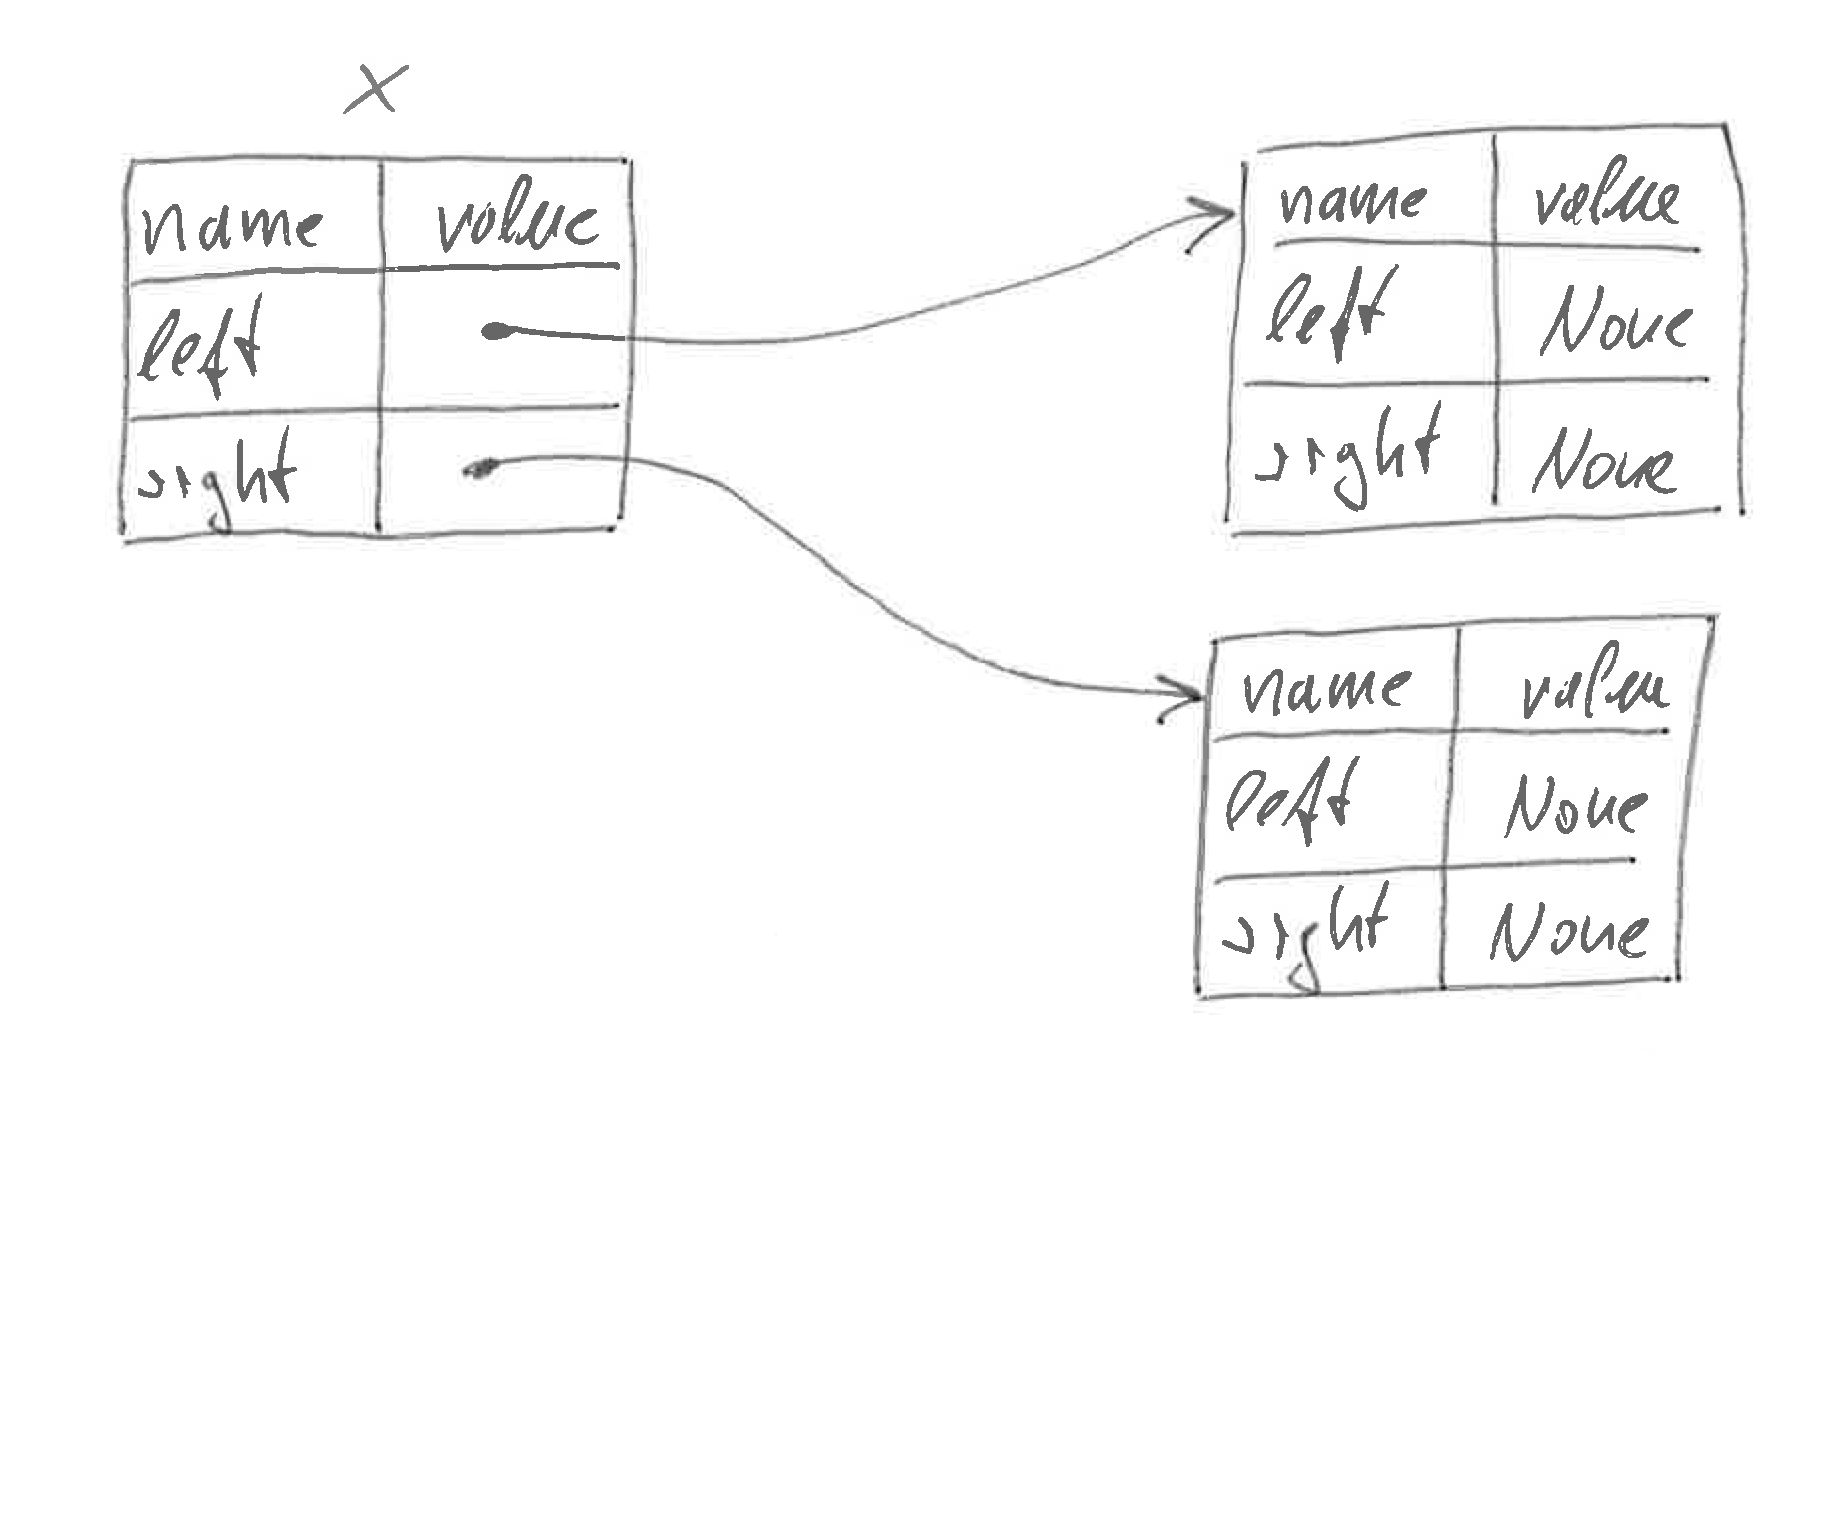
\includegraphics[width=8cm]{content/chapter_rust_depth/tree-1}}%
    \only<2>{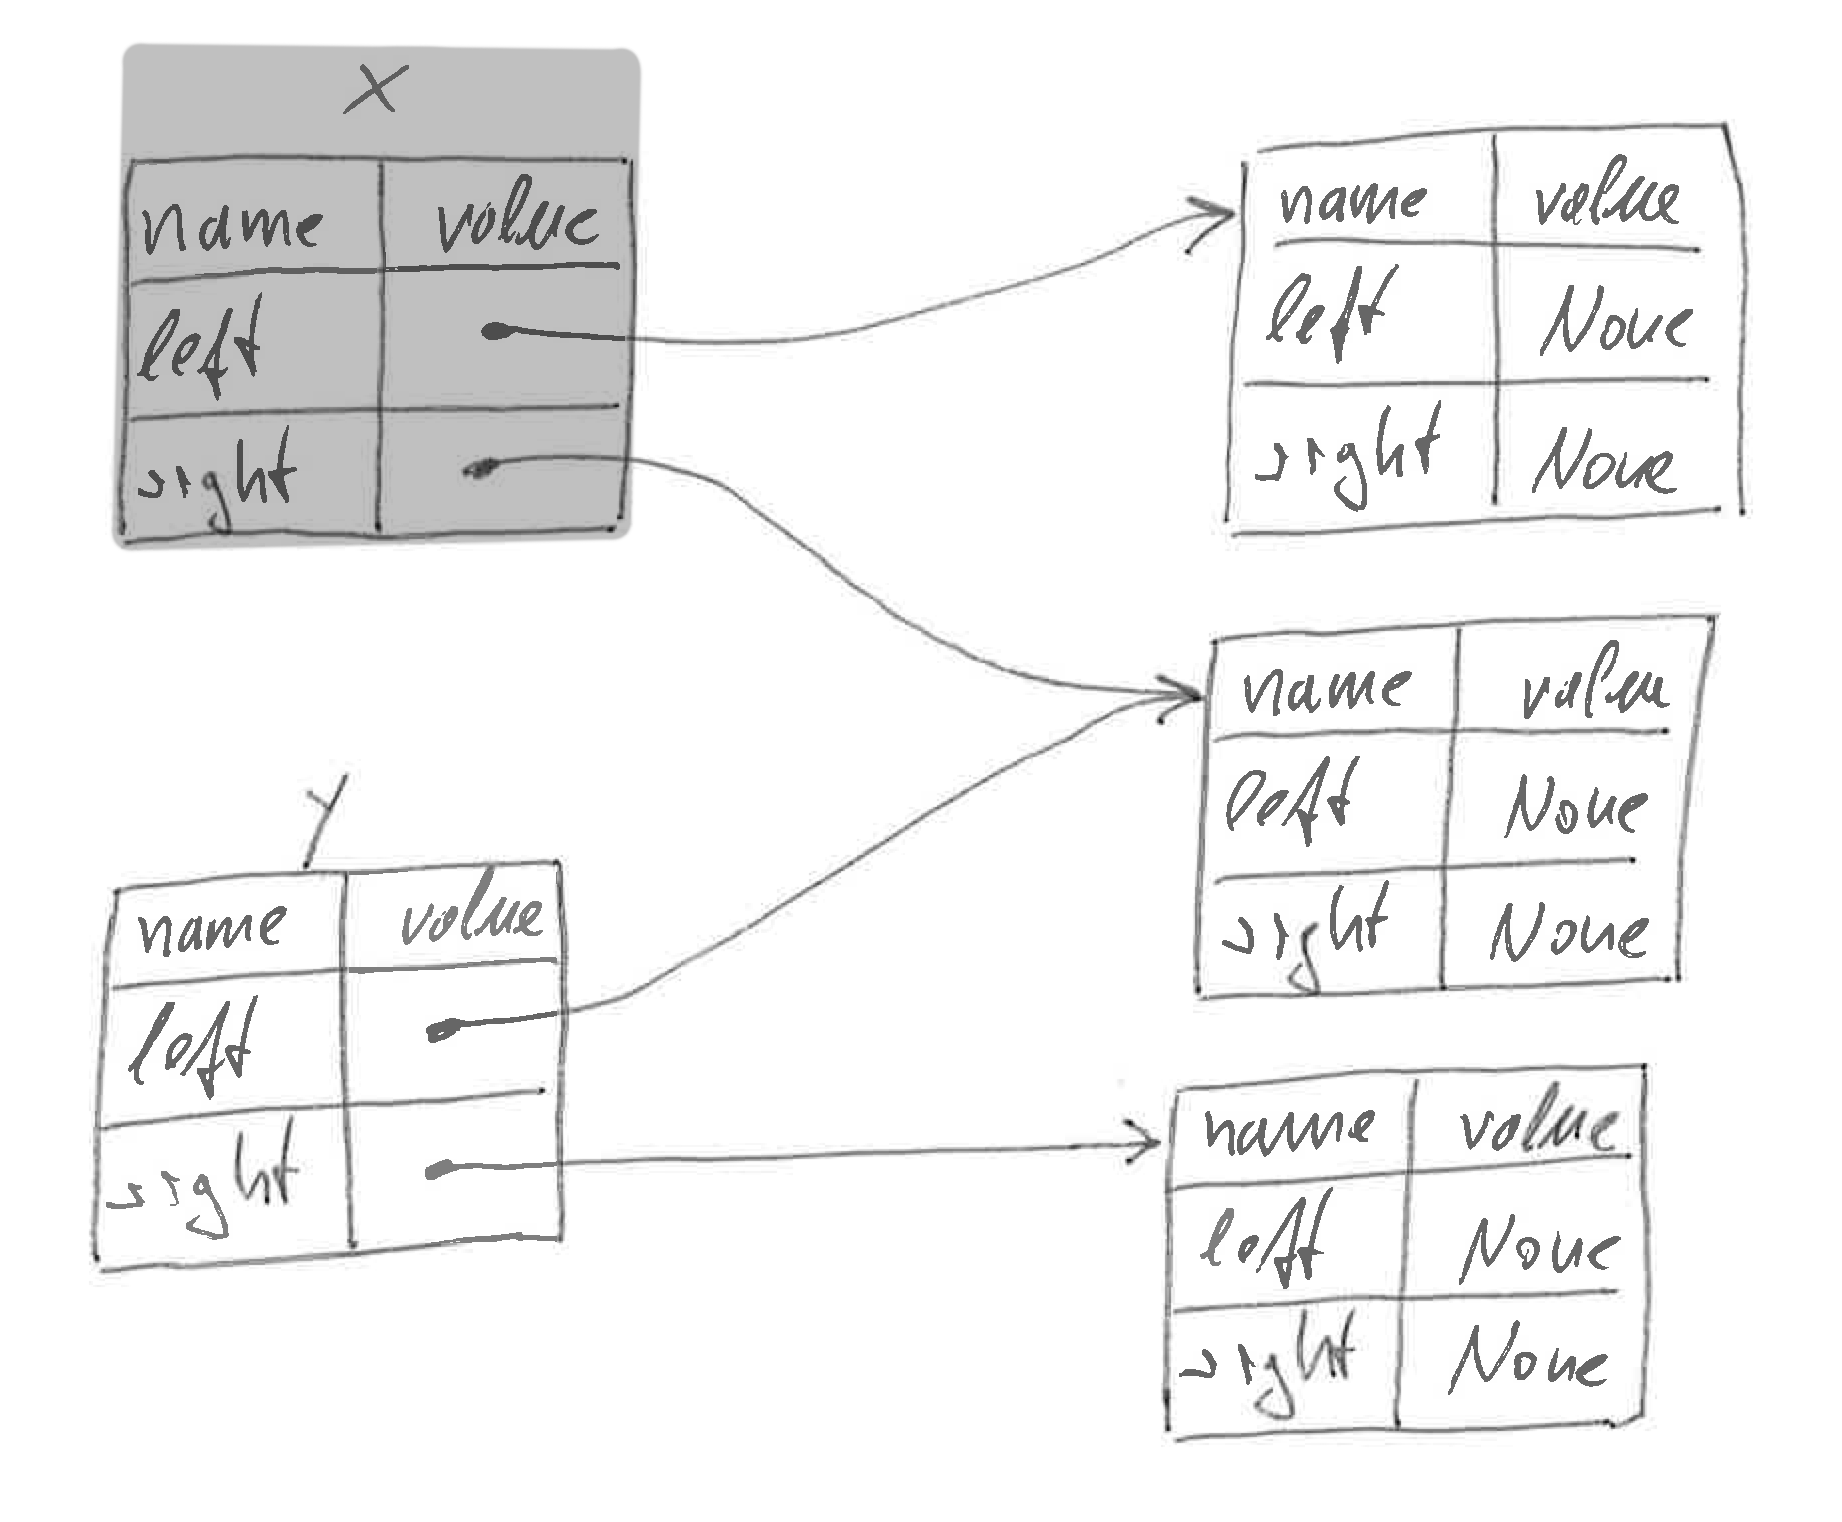
\includegraphics[width=8cm]{content/chapter_rust_depth/tree-2}}%
  }
\end{Frame}

\section{Lifetime}

\subsection{Working}

\begin{Frame}[fragile]{Lifetime in C: Working}
\begin{lstlisting}[language=C]
struct Node {
    struct Node* left;
    struct Node* right;
};

void works() {
    struct Node left_child = {NULL, NULL};
    struct Node right_child = {NULL, NULL};
    struct Node parent = {&left_child, &right_child};
    do_something(&parent);
}
\end{lstlisting}
\end{Frame}

\begin{Frame}[fragile]{Lifetime in Rust: Working}
\begin{lstlisting}[language=Rust]
struct Node<'a> {
    left: Option<&'a Node<'a>>,
    right: Option<&'a Node<'a>>
}

impl <'a> Node<'a> {
    fn empty() -> Node<'a> {
        Node {left: None, right: None}
    }
}

fn works() {
    let left_child = Node::empty();
    let right_child = Node::empty();
    let parent = Node {left: Some(&left_child),
                       right: Some(&right_child)};
    do_something(&parent);
}
\end{lstlisting}
\end{Frame}

\subsection{Dangling Pointer}

\begin{Frame}[fragile]{Lifetime in C: Dangling Pointer}
\begin{lstlisting}[language=C]
struct Node {
    struct Node* left;
    struct Node* right;
};

void does_not_work(bool should_create_children) {
    struct Node parent;
    if (should_create_children) {
        struct Node left_child = {0};
        struct Node right_child = {0};
        parent.left = &left_child;
        parent.right = &right_child;
    } else {
        parent.left = parent.right = NULL;
    }
    do_something(&parent); // WRONG!
    // left_child's and right_child's lifetime end at
    // the end of the block, so parent now contains
    // dangling pointers if `should_create_children`
}
\end{lstlisting}
\end{Frame}

\begin{Frame}[fragile]{Lifetime in Rust: Compile Error}
\begin{lstlisting}[language=Rust]
struct Node<'a> {
    left: Option<&'a Node<'a>>,
    right: Option<&'a Node<'a>>
}

impl <'a> Node<'a> {
    fn empty() -> Node<'a> {
        Node {left: None, right: None}
    }
}

fn does_not_work(should_create_children: bool) {
    let mut parent = Node::empty();
    if should_create_children {
        let left_child = Node::empty();
        let right_child = Node::empty();
        parent = Node {left: Some(&left_child),
                       right: Some(&right_child)}; // ERROR!
        // `left_child` does not live long enough
        // and
        // `right_child` does not live long enough
    }
    do_something(&parent);
}
\end{lstlisting}
\end{Frame}

\section*{Conclusion}

\begin{frame}{Conclusion}
  \begin{enumerate}
    \item Rust's type system \alert{can prevent some common errors}, e.g. concurrent or accidental modification, dangling pointers or double frees, \ldots
    \item Rust \alert{enforces} the following rules:
      \begin{itemize}
        \item For every memory object there is \alert{exactly one owner}.
        \item At any given time, you can have \alert{either one mutable reference or any number of immutable references}.
        \item References must always be valid.
        \item Mutability must always be explicitly encoded in the type.
      \end{itemize}
    \item Following these rules \alert{might take longer}, but \alert{might lead to safer code}.
  \end{enumerate}
\end{frame}
